\documentclass[12pt, a4paper, twoside]{article} %Dokumentenklasse Setzen

\usepackage[a4paper, left=2.5cm, right=2.5cm]{geometry} %Seitenrand setzen

\usepackage[T1]{fontenc}
\usepackage{lmodern}
\usepackage{textcomp}
\usepackage[utf8]{inputenc}
\usepackage[ngerman]{babel}
\usepackage[ngerman]{babel}
\usepackage{csquotes}
\usepackage{xpatch}
\usepackage{xspace} % setzten von Leerzeichen nach Abkürzungen
\usepackage{microtype} % für glättere Seitenränder

\usepackage{fancyhdr} % für schöne Header
\pagestyle{fancy}
\fancyhf{}
\fancyhead[R]{\rightmark}
\fancyfoot[LE]{\thepage}
\fancyfoot[RO]{\thepage}
\renewcommand{\headrulewidth}{0.4pt}
\renewcommand{\footrulewidth}{0.4pt}

% Abkürzungspaket
\usepackage{acronym}

% Mathe Pakete
\usepackage{amsmath}
\usepackage{thmtools}
\usepackage{amsfonts}
\usepackage{amssymb}

% Listenumgebungen
\usepackage{listings}
\usepackage{paralist}
\usepackage{enumitem}
\usepackage{adjustbox}

% Demo Text
\usepackage{blindtext}

% Farb-Pakete
\usepackage[dvipsnames]{xcolor}
\usepackage{colortbl}
% Farbedefinitionen
\definecolor{htw}{RGB}{120, 184, 2}

% Für erweiterte Tabellen
\usepackage{longtable}
\usepackage{float}
\usepackage{multirow}
\usepackage{makecell}
\usepackage{cellspace}
\setlength{\tabcolsep}{0.5em} % for the horizontal padding
{\renewcommand{\arraystretch}{1.8} % for the vertical padding
\usepackage{ragged2e}
\newcolumntype{R}[1]{>{\RaggedRight}p{#1}}

% Für Einheiten
\usepackage[exponent-product = \cdot]{siunitx}
\sisetup{locale=DE}

\makeatletter
\renewcommand\@dotsep{5}
\makeatother

% Pakete für Grafiken
\usepackage{graphicx}
\usepackage{wrapfig}
\usepackage{epstopdf}
\usepackage{subcaption}
%\captionsetup[subfigure]{list=true, font=normalsize, labelformat=brace, position=top} %setup für subfigure captions
\usepackage{pstricks}
\usepackage{tikz}
\usepackage{tikz-uml}
\usepackage{pgfkeys}
\usepackage{pgfopts}
\usepackage{ifthen}
\usepackage{xstring}
\usepackage{calc}
\usepackage{pst-plot,pst-bar} % Balkendiagramme
\usepackage{capt-of}
\usepackage{incgraph} % Fullscreen Images
\usepackage{pdfpages} % Include external pdf pages

% Paket für Literaturverzeichnis
\usepackage[
    style=alphabetic,
    sorting=nty,
    sortcites=true,
    autopunct=true,
    autolang=hyphen,
    hyperref=true,
    abbreviate=false,
    backref=true,
    backend=biber,
    block=space
    ]{biblatex}

\addbibresource{bib/bib.bib} %Einfügen der Literaturbibliothek
\defbibheading{bibempty}{}


\usepackage{url}
\usepackage{hyperref}
\hypersetup{hidelinks}
\urlstyle{same}

%Abkürzungen durch Kommandos setzen
\newcommand{\bspw}{bspw.\xspace}
\newcommand{\bzw}{bzw.\xspace}
\newcommand{\etc}{etc.\xspace}
\newcommand{\zB}{z.\,B.\xspace}
\newcommand{\EV}{e.\,V.\xspace}
\newcommand{\zT}{z.\,T.\xspace}
\newcommand{\iVm}{i.\,V.\,m.\xspace}
\newcommand{\idR}{i.\,d.\,R.\xspace}
\newcommand{\ihv}{i.\,H.\,v.\xspace}
\newcommand{\ua}{u.\,a.\xspace}
\newcommand{\dH}{d.\,h.\xspace}
\newcommand{\vgl}{vgl.\xspace}
\newcommand{\ca}{ca.\xspace}
\newcommand{\dV}{d.\,Verf.}
\newcommand{\RNr}{Rn.\xspace}
\newcommand{\oa}{o.\,{ä}.\xspace}
\newcommand{\vC}{v.\,Chr.\xspace}
\newcommand{\nC}{n.\,Chr.\xspace}
\newcommand{\vA}{v.\,a.\xspace}
\newcommand{\eng}{engl.\xspace}
\newcommand{\tabitem}{~~\llap{\textbullet}~~}

\newcommand{\fakesection}[1]{%
  \par\refstepcounter{section}% Increase section counter
  \sectionmark{#1}% Add section mark (header)
  \addcontentsline{toc}{section}{\protect\numberline{\thesection}#1}% Add section to ToC
  % Add more content here, if needed.
}

\usepackage[nottoc,numbib]{tocbibind}
% \usepackage{tocbibind} % damit Verzeichnisse im Inhaltsverzeichnis aufgeführt werden
% \usepackage[nottoc]{tocbibind} % damit Inhaltsverzeichnis nicht im Inhaltsverzeichnis vorkommt

\usepackage{subfiles} % Best loaded last in the preamble

\pagenumbering{Roman} %Römische Seitennummerierung für Verzeichnisse

\begin{document}

%TITELSEITE
\begin{titlepage}

	\vspace*{-2.0cm}

	\begin{figure}[h]\centering
		
\includegraphics[width=5cm]{Images/HTW_Logo.png}
	\end{figure}

	\begin{center}
	\vspace*{-1.59cm}

	\par\noindent\rule{\textwidth}{0.4pt}
	\huge
	\textcolor{htw}{\textbf{Konzeption, Projektierung und Inbetriebnahme eines mehrachsigen Positioniersystems}}
	\par\noindent\rule{\textwidth}{0.4pt}
	\vspace*{2.0cm}
	\Large
	Bachelorarbeit
	
	\normalsize
	Name des Studiengangs\\
	\vspace*{0.4cm}
	\Large
	Elektrotechnik
	
	\vspace*{0.6cm}
	\Large
	\textcolor{htw}{Fachbereich 1}
	
	\vspace*{0.6cm}
	\normalsize
	vorgelegt von\\
	\vspace*{0.4cm}
	\Large
	Aaron Zielstorff
	
	\vspace*{3.0cm}
	\small
	Datum:\\
	\normalsize
	Berlin, 20.10.2021
	
	\vspace*{1.6cm}
	\normalsize
	Erstgutachter\textunderscore in: Herr Prof. Dr. Stephan Schäfer\\
	Zweitgutachter\textunderscore in: Herr Dipl.-Ing. Dirk Schöttke
	
	\end{center}
\end{titlepage}


%INHALTSVERZEICHNIS
\pagestyle{empty}
\setcounter{tocdepth}{3} %Inhaltsverzeichnis zeigt 3 Gliederungsebenen
\tableofcontents
\clearpage

% Aufgabenstellung
\addcontentsline{toc}{section}{Aufgabenstellung}
% \color{red}
% Aufgabenstellung aus PDF vom Prüfungsamt übernehmen!!!
% \color{black}
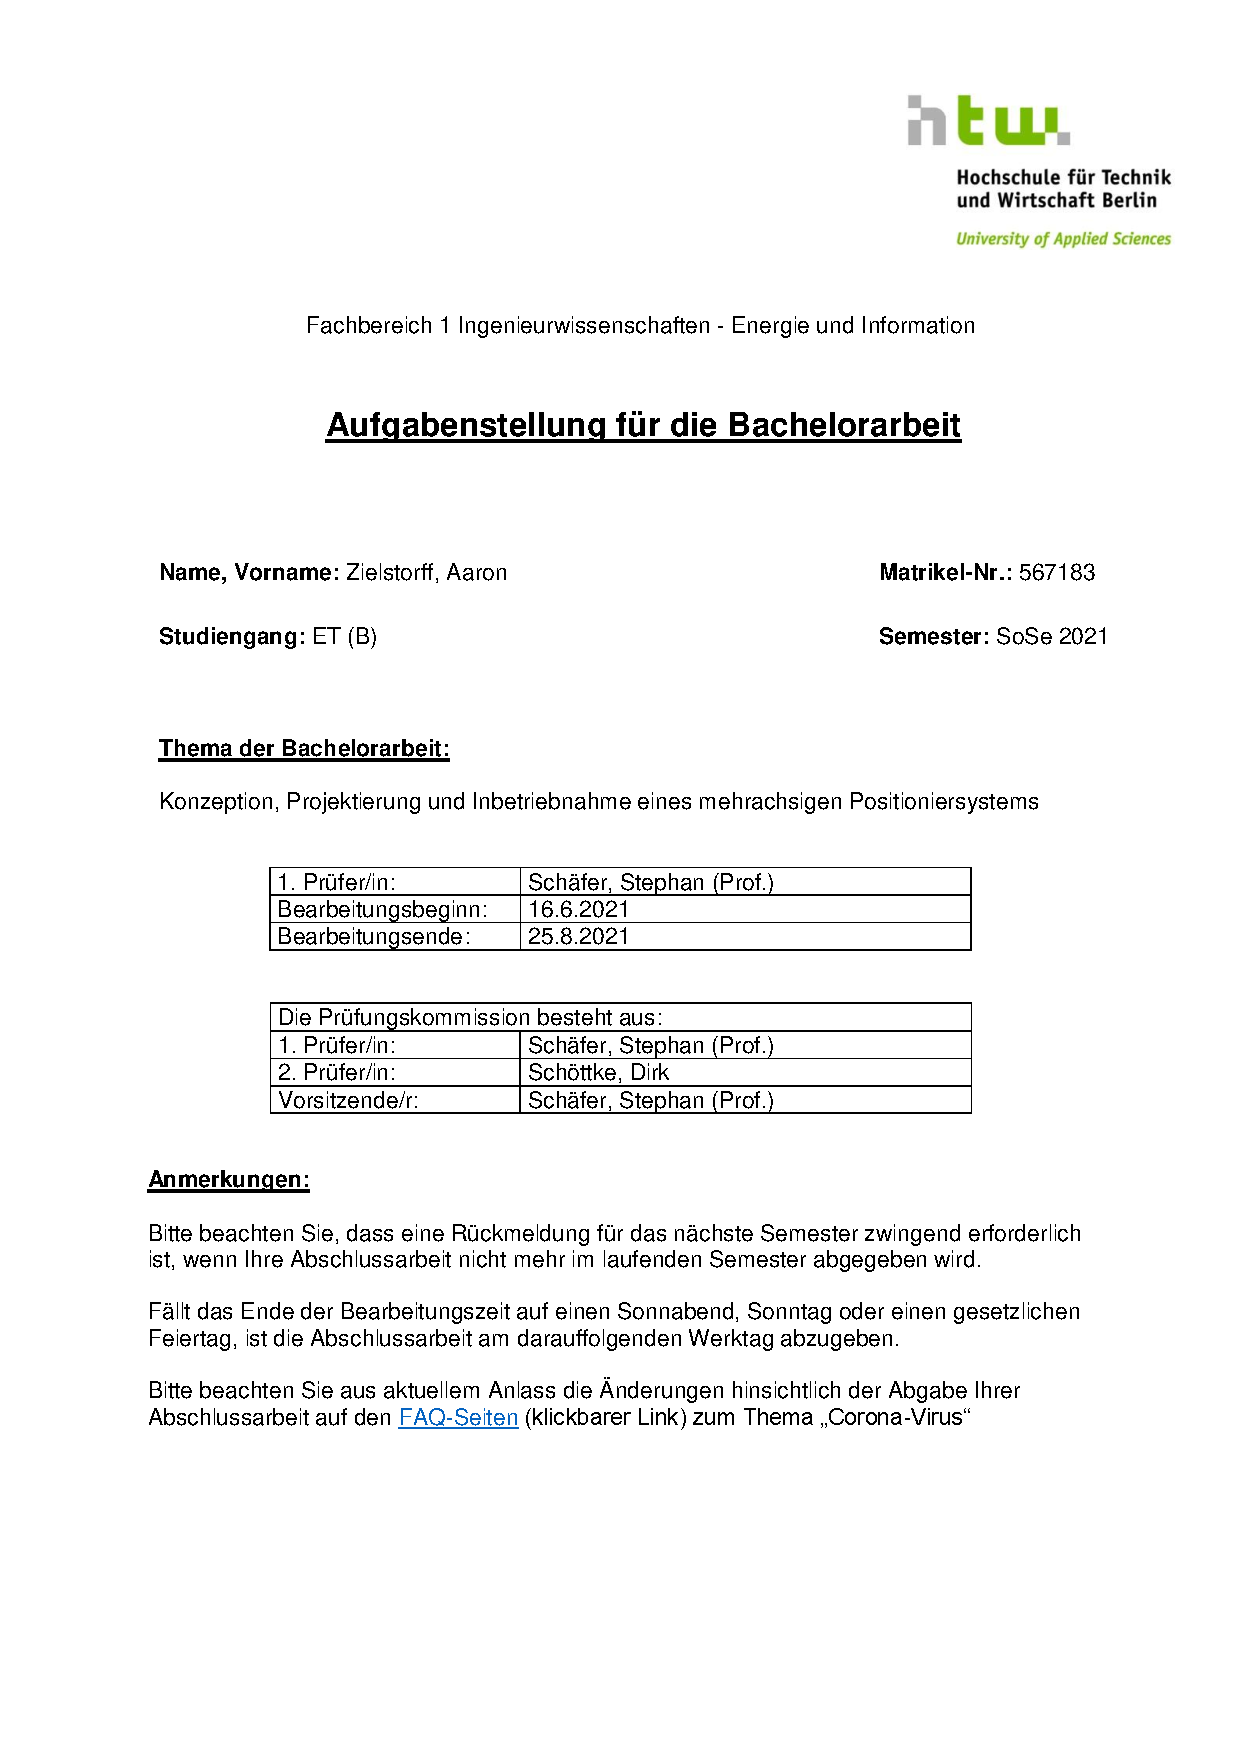
\includepdf{Images/Aufgabenstellung.pdf}
\clearpage

% ABBILDUNGSVERZEICHNIS
\listoffigures
\clearpage

% TABELLENVERZEICHNIS
\listoftables
\clearpage

% ABKÜRZUNGSVERZEICHNIS
\section*{Abkürzungsverzeichnis}
\addcontentsline{toc}{section}{Abkürzungsverzeichnis}
\begin{acronym}[FA]
	\acro{fa}[FA]{Funktionale Anforderung}
	\acroplural{fa}[FAs]{Funktionale Anforderungen}
	\acro{nfa}[NFA]{Nicht-Funktionale Anforderung}
	\acroplural{nfa}[NFAs]{Nicht-Funktionale Anforderungen}
\end{acronym}
\begin{acronym}[VR]
	\acro{ar}[AR]{Augmented Reality}
	\acro{vr}[VR]{Virtual Reality}
\end{acronym}
\begin{acronym}[HMI]
	\acro{hmi}[HMI]{Human Machine Interface}
	\acro{mms}[MMS]{Mensch-Maschine-Schnittstelle}
\end{acronym}
\begin{acronym}[LMC]
	\acro{lmc}[LMC]{Logic Motion Controller}
	\acro{lxm}[LXM]{Lexium}
\end{acronym}
\begin{acronym}[OPC]
	\acro{opc}[OPC]{Open Plattform Communications}
	\acro{ua}[UA]{Unified Architecture}
\end{acronym}
\begin{acronym}[ID]
	\acro{id}[ID]{Identifikationsnummer}
\end{acronym}
\begin{acronym}[SPS]
	\acro{sps}[SPS]{speicherprogrammierbare Steuerung}
	\acroplural{sps}[SPSen]{speicherprogrammierbare Steuerungen}
\end{acronym}
\begin{acronym}[HTW]
	\acro{htw}[HTW]{Hochschule für Technik und Wirtschaft}
\end{acronym}
\begin{acronym}[UML]
	\acro{uml}[UML]{Unified Modeling Language}
\end{acronym}
\begin{acronym}[RE]
	\acro{re}[RE]{Requierements Engineering}
\end{acronym}
\begin{acronym}[BMK]
	\acro{bmk}[BMK]{Betriebsmittelkennung}
\end{acronym}
\begin{acronym}[EA]
	\acro{ea}[E/A]{Eingang/Ausgang}
\end{acronym}
\begin{acronym}[TA]
	\acro{ta}[TA]{Taster}
\end{acronym}
\begin{acronym}[RTG]
	\acro{rtg}[Rtg.]{Richtungsgeber}
\end{acronym}
\begin{acronym}[NA]
	\acro{na}[NA]{nicht angeschlossen}
\end{acronym}
\begin{acronym}[Poti]
	\acro{poti}[Poti]{Potentiometer}
\end{acronym}
\begin{acronym}[SLC]
	\acro{slc}[SLC]{Safety Logic Controller}
\end{acronym}
\begin{acronym}[GUI]
	\acro{gui}[GUI]{Graphical User Interface}
\end{acronym}
\begin{acronym}[TF]
	\acro{tf}[TF]{Testfall}
\end{acronym}
\begin{acronym}[KI]
	\acro{ki}[KI]{künstliche Intelligenz}
\end{acronym}
\clearpage

\pagestyle{fancy}
\pagenumbering{arabic} %Arabische Seitennummerierung nach den ab Textbeginn

% Einleitung
\subfile{sections/01_Einleitung/einleitung.tex}

% Theoretische Grundlagen
% \newpage
% \subfile{sections/02_TheoretischeGrundlagen/theoGrundl.tex}

% \subfile{sections/02_TheoretischeGrundlagen/1_RequirementsEngineering/RequirementsEngineering.tex}

% \newpage
% \subfile{sections/02_TheoretischeGrundlagen/2_Anlagenprojektierung/Anlagenprojektierung.tex}

% Konzeption
\newpage
\subfile{sections/03_Konzeption/konzeption.tex}

\subfile{sections/03_Konzeption/1_Anforderungsanalyse/AnforderungsAna.tex}

\newpage
\subfile{sections/03_Konzeption/2_Stakeholder/Stakeholder.tex}

\newpage
\subfile{sections/03_Konzeption/3_Laboranlage/Laboranlage.tex}

\newpage
\subfile{sections/03_Konzeption/4_Bedienkonzept/Bedienkonzept.tex}

% Projektierung
\newpage
\subfile{sections/04_Projektierung/projektierung.tex}


\subfile{sections/04_Projektierung/1_Kontextanalyse/Kontextanalyse.tex}

\newpage
\subfile{sections/04_Projektierung/2_AnwendungsfallSpez/AnwendungsfallSpez.tex}

\newpage
\subfile{sections/04_Projektierung/3_VerhaltensSpez/VerhaltensSpez.tex}

\newpage
\subfile{sections/04_Projektierung/4_Partitionierung/Partitionierung.tex}

\newpage
\subfile{sections/04_Projektierung/5_Testspezifikation/Testspezifikation.tex}

\newpage
\subfile{sections/04_Projektierung/6_Stromlaufplan/Stromlaufplan.tex}

\newpage
\subfile{sections/04_Projektierung/7_Datenmodell/Datenmodell.tex}

\newpage
\subfile{sections/04_Projektierung/8_Sicherheit/sicherheit.tex}

% Inbetriebnahme
\newpage
\subfile{sections/05_Inbetriebnahme/Inbetriebnahme.tex}

\subfile{sections/05_Inbetriebnahme/1_Implementation/Implementation.tex}

\newpage
\subfile{sections/05_Inbetriebnahme/2_Testueberpruefung/Testueberpruefung.tex}

\newpage
\subfile{sections/05_Inbetriebnahme/3_Korrektur/Korrektur.tex}

%\newpage
%\subfile{sections/05_Inbetriebnahme/4_Bedienung/Bedienung.tex}

% Fazit
\newpage
\subfile{sections/06_Fazit/fazit.tex}

% Ausblick
\newpage
\subfile{sections/07_Ausblick/ausblick.tex}

\newpage
\section*{Literaturverzeichnis}
\addcontentsline{toc}{section}{Literaturverzeichnis}

\nocite{Laplante2014}
\nocite{Bindel2017}
\nocite{Kleuker2013}
\nocite{Keller2019}
\nocite{John2009}
\nocite{Heinrich2019}
\nocite{Abolhassan2016}
\nocite{Commission1998}
\nocite{Andelfinger2017}
\nocite{Lauber1999}
\nocite{Walke2005}
\nocite{Marwedel2007}
\nocite{Broy2021}
\nocite{Balzert2009}
\nocite{Tabeling2006}
\nocite{Goll2011}
\nocite{Wietzke2012}

\printbibliography[
	heading=subbibintoc,
	type=book,
	title={Bücher}
]

\nocite{t2info2012}

\printbibliography[
	heading=subbibintoc,
	type=article,
	title={Artikel}
]

% Anhang
\newpage
\subfile{sections/anhang.tex}

% Eidesstattliche Erklärung
\newpage
\subfile{sections/eidesstattlicheErklaerung.tex}

\end{document}